\begin{explanationbox}
\textbf{\textcolor{CExplanation}{阅读顺序：先圆，后公式；先知道为什么有用，再记名称。}}

\medskip
\textbf{\textcolor{CExplanation}{一、为什么会发明“点配一条直线”这种做法？}}

先看圆 $x^2+y^2=4$。在圆外取 $P(4,0)$，从 $P$ 作两条切线，分别与圆相切于 $T,T'$。圆心 $O(0,0)$ 到切点的半径垂直于切线，因此两个切点都满足
\[
\underbrace{4x_{T}+0y_{T}}_{\text{把切点坐标代入}}=4,
\qquad\text{即}\quad x_T=1.
\]
所以两切点的连线是 $x=1$。把这一条直线与原来的点 $P$ 对应起来，就有了最初的直观认识：\textbf{圆外点的极线，就是两个切点的连线。}

\begin{center}
\begin{tikzpicture}[x=1.2cm,y=1.2cm,every node/.style={font=\small}]
\coordinate (O) at (0,0); \coordinate (P) at (4,0);
\coordinate (T) at (1,{sqrt(3)}); \coordinate (U) at (1,{-sqrt(3)});
\draw[blue!75!black,thick] (O) circle (2);
\draw[gray!70] (O)--(P) (O)--(U);
\draw[orange!80!black,thick] (P)--(T) (P)--(U);
\draw[gray!80,thick] (O)--(T) node[midway,above left] {$r$};
\draw[red!75!black,dashed,thick] (1,-2.2)--(1,2.3);
\draw ($(T)!.16!(O)$)--($(T)!.16!(O)+(.277128,-.16)$)--($(T)+(.277128,-.16)$);
\fill (O) circle (1.8pt) node[below left] {$O$};
\fill (P) circle (2pt) node[below right] {$P$};
\fill (T) circle (2pt) node[above right] {$T(x,y)$};
\fill (U) circle (2pt) node[below right] {$T'$};
\node[red!75!black,above] at (1,2.3) {$l_P=TT'$};
\node at (1,-2.9) {$OT\perp PT\quad\Longrightarrow\quad OP^2=OT^2+PT^2$};
\end{tikzpicture}

\end{center}
\textbf{看图要注意：} $T,T'$ 位于圆上；$PT,PT'$ 才是切线段；红色虚线 $TT'$ 是\textbf{切点弦}，不是从 $P$ 引出的切线。这个区别很重要。

\medskip
\textbf{\textcolor{CExplanation}{二、圆外、圆上、圆内，为什么能用同一条公式？}}

对任何\textbf{不是圆心}的点 $R(u,v)$，先写出同一个方程
\[
\boxed{l_R:\ ux+vy=4}.
\]
不要一开始纠结“为什么必须叫极线”。先把它当成\textbf{一条按相同规则得到的直线}，分别看三种情况：

\begin{center}
\begin{tikzpicture}[x=.52cm,y=.52cm,every node/.style={font=\small}]
\foreach \shift/\u/\v/\title/\eq in {0/4/1/圆外：切点弦/{x=1},8.6/2/2/圆上：切线/{x=2},17.2/1/4/圆内：对应直线/{x=4}} {
\begin{scope}[xshift=\shift*.52cm]
\draw[->,gray!60] (-2.4,0)--(4.7,0);
\draw[blue!75!black,thick] (0,0) circle (2);
\draw[red!75!black,dashed,thick] (\v,-2.5)--(\v,2.5);
\fill (\u,0) circle (2pt);
\node[align=center] at (1,3.8) {\title\\$R(\u,0)$};
\node[red!75!black] at (1,-4.2) {$l_R:\eq$};
\end{scope}}
\draw[orange!80!black,thick] (4,0)--(1,{sqrt(3)}) (4,0)--(1,{-sqrt(3)});
\fill (1,{sqrt(3)}) circle (1.7pt); \fill (1,{-sqrt(3)}) circle (1.7pt);
\node at (9.5,-5.8) {同一圆、同一尺度：$ux+vy=4$；圆内点不能引出真实切线。};
\end{tikzpicture}

\end{center}
\textbf{沿图比较：} $R$ 从 $(4,0)$ 移至 $(2,0)$、$(1,0)$ 时，极线依次为 $x=1,2,4$；它与圆依次有两个、一个、零个交点。\textbf{变的是位置与几何含义，配线公式没有变。}

这里的“统一”是\textbf{用同一个代数方程处理不同位置的点}，不等于说圆内点也能作两条切线。这正是新概念值得引入的原因：\textbf{几何图形的情况会变，方程却保持一个样子。}

\medskip
\textbf{\textcolor{CExplanation}{三、最值得理解的发现：点在线上动，线却经过定点}}

继续取圆 $x^2+y^2=4$ 和固定点 $P(4,0)$。已经知道
\[
 l_P:x=1.
\]
在 $x=1$ 上任取 $Q(1,t)$，$t$ 可以是任何实数。按照上面的统一规则，点 $Q$ 配出的直线为
\[
\boxed{l_Q:\ x+ty=4}.
\]
\textbf{检验：} 把固定点 $P(4,0)$ 代入 $l_Q$ 的左边，得到 $4+t\cdot0=4$，对任意 $t$ 都成立。因此 $l_Q$ 始终经过 $P$，哪怕 $Q$ 处在圆内、圆上或圆外。

\begin{center}
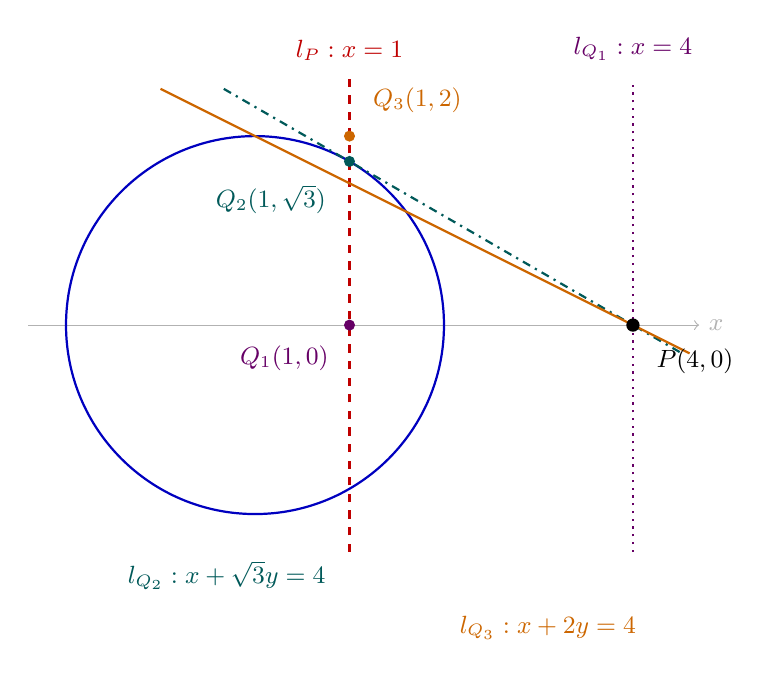
\begin{tikzpicture}[x=1.2cm,y=1.2cm,every node/.style={font=\small}]
\draw[->,gray!60] (-2.4,0)--(4.7,0) node[right] {$x$};
\draw[blue!75!black,thick] (0,0) circle (2);
\draw[red!75!black,dashed,thick] (1,-2.4)--(1,2.6);
\draw[violet!80!black,thick,dotted] (4,-2.4)--(4,2.6);
\draw[teal!70!black,thick,dash dot] ({4-2.5*sqrt(3)},2.5)--(4.5,{-0.5/sqrt(3)});
\draw[orange!80!black,thick] (-1,2.5)--(4.6,-.3);
\fill (4,0) circle (2.4pt) node[below right=5pt] {$P(4,0)$};
\fill[violet!80!black] (1,0) circle (2pt) node[below left=4pt] {$Q_1(1,0)$};
\fill[teal!70!black] (1,{sqrt(3)}) circle (2pt) node[below left=5pt] {$Q_2(1,\sqrt3)$};
\fill[orange!80!black] (1,2) circle (2pt) node[above right=5pt] {$Q_3(1,2)$};
\node[red!75!black,above] at (1,2.7) {$l_P:x=1$};
\node[violet!80!black,above] at (4,2.7) {$l_{Q_1}:x=4$};
\node[teal!70!black] at (-.3,-2.65) {$l_{Q_2}:x+\sqrt3y=4$};
\node[orange!80!black] at (3.1,-3.2) {$l_{Q_3}:x+2y=4$};
\end{tikzpicture}

\end{center}
\textbf{画图说明：} 紫色 $l_{Q_1}$ 为 $x=4$；青色 $l_{Q_2}$ 为 $x+\sqrt3y=4$；橙色 $l_{Q_3}$ 为 $x+2y=4$。三条直线都经过 $P$。切点弦所对应的直线一般\textbf{并不经过动点 $Q_3$ 本身}。

\textbf{进一步观察：}
\begin{itemize}[leftmargin=*,itemsep=0.38em]
\item $Q_1=(1,0)$ 在圆内；$l_{Q_1}:x=4$ 与圆没有交点。
\item $Q_2=(1,\sqrt3)$ 在圆上；$l_{Q_2}:x+\sqrt3y=4$ 是此处的切线。
\item $Q_3=(1,2)$ 在圆外；$l_{Q_3}:x+2y=4$ 是从 $Q_3$ 作两条切线时两个切点的连线。
\end{itemize}
所以：“极线”的价值并非又多记一个名字，而是\textbf{把三种画法完全不同的点统一到一条简单公式，并由此发现动线过定点。}

\medskip
\textbf{\textcolor{CExplanation}{四、为什么交换 $P$、$Q$ 一定成立？}}

设圆上统一方程为 $x^2+y^2=r^2$，$P(x_1,y_1)$ 与 $Q(x_2,y_2)$ 均不是圆心。
\[
\begin{aligned}
Q\in l_P &\iff x_1x_2+y_1y_2=r^2,\\
P\in l_Q &\iff x_2x_1+y_2y_1=r^2.
\end{aligned}
\]
左边两式只是乘法顺序颠倒：$x_1x_2=x_2x_1$、$y_1y_2=y_2y_1$。因此两者必然同时成立或同时不成立。\textbf{这只是乘法交换律，不是高深理论。}

\medskip
\textbf{\textcolor{CExplanation}{五、椭圆、双曲线、抛物线也一样吗？}}

是的。只看每一类曲线判断 $Q$ 在 $l_P$ 上需要满足什么等式：
\begin{itemize}[leftmargin=*,itemsep=0.4em]
\item 椭圆：$\displaystyle \frac{x_1x_2}{a^2}+\frac{y_1y_2}{b^2}=1$；交换下标 $1,2$ 不变。
\item 双曲线：$\displaystyle \frac{x_1x_2}{A^2}-\frac{y_1y_2}{B^2}=1$；减号不影响乘法交换律。
\item 抛物线：$\displaystyle y_1y_2=p(x_1+x_2)$；左边乘法可交换，右边加法也可交换。
\end{itemize}

\begin{center}
\begin{tikzpicture}[every node/.style={font=\small}]
\begin{scope}[x=1cm,y=1cm]
\draw[->,gray!60] (-2.4,0)--(2.8,0) node[right] {$x$};
\draw[->,gray!60] (0,-1.4)--(0,1.7) node[above] {$y$};
\draw[blue!75!black,thick] (0,0) ellipse (2 and 1);
\draw[red!75!black,dashed,thick] (2,-1.3)--(2,1.4);
\fill (2,0) circle (2pt);\node[anchor=west] at (2.15,-.6) {$P(2,0)$};
\fill (2,1) circle (2pt) node[right=4pt] {$Q(2,1)$};
\node at (0,-2) {$x^2/4+y^2=1$};
\end{scope}
\draw[->,thick,gray] (3,.3)--(5,.3) ;\node[align=center,gray] at (4,1.7) {$X=x/2$\\$Y=y$};
\begin{scope}[xshift=7.5cm,x=1cm,y=1cm]
\draw[->,gray!60] (-1.5,0)--(2.3,0) node[right] {$X$};
\draw[->,gray!60] (0,-1.4)--(0,1.7) node[above] {$Y$};
\draw[blue!75!black,thick] (0,0) circle (1);
\draw[red!75!black,dashed,thick] (1,-1.3)--(1,1.4);
\fill (1,0) circle (2pt);\node[anchor=west] at (1.15,-.6) {$P'(1,0)$};
\fill (1,1) circle (2pt) node[right=4pt] {$Q'(1,1)$};
\node at (0,-2) {$X^2+Y^2=1$};
\end{scope}
\node at (3.8,-2.8) {左右每格均为 $1$；只把横坐标减半，点在线上的关系保留。};
\end{tikzpicture}

\end{center}
\textbf{由图推广：} 对 $x^2/a^2+y^2/b^2=1$，令 $X=x/a,Y=y/b$，就得到单位圆；点也同时改坐标。将单位圆极线 $X_1X+Y_1Y=1$ 改回原坐标，便得
\[
\boxed{\frac{x_1x}{a^2}+\frac{y_1y}{b^2}=1}.
\]
图中直线 $x=2$ 变成 $X=1$，点仍在对应直线上。这正是配线公式随坐标一起改变的含义。

遇到这些题目，一般\textbf{没有必要}先记住一个新的字母 $S_P$；看原来曲线的具体方程，把对应点坐标放进去就够了。

\medskip
\par\medskip\noindent\begin{minipage}{\linewidth}
\textbf{\textcolor{CExplanation}{六、同一点坐标，换曲线就要换公式}}
\begin{center}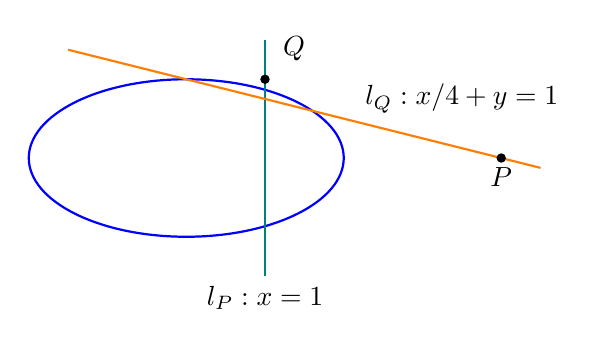
\begin{tikzpicture}[scale=1.0,>=stealth]
\draw[blue,thick] (0,0) ellipse (2 and 1);\draw[teal,thick] (1,-1.5)--(1,1.5);\draw[orange,thick] (-1.5,1.375)--(4.5,-.125);\fill (4,0) circle (1.7pt) node[below] {$P$};\fill (1,1) circle (1.7pt) node[above right=3pt] {$Q$};\node[below] at (1,-1.5) {$l_P:x=1$};\node[above] at (3.5,.45) {$l_Q:x/4+y=1$};
\end{tikzpicture}
\end{center}
这里使用的是椭圆 $\dfrac{x^2}{4}+y^2=1$，不是上面半径为 $2$ 的圆。$P=(4,0)$ 的极线是 $x=1$，$Q=(1,1)$ 的极线是 $\dfrac{x}{4}+y=1$。验证：$Q$ 满足 $x=1$；把 $P$ 代入 $\frac{x}{4}+y=1$，得 $\frac44+0=1$。\textbf{圆的公式与椭圆的公式不可混用。}
\end{minipage}\par

\medskip
\textbf{\textcolor{CExplanation}{七、考场上怎么决定用不用？}}
\begin{itemize}[leftmargin=*,itemsep=0.4em]
\item \textbf{识别信号：} 两条切线、两个切点、切点弦、某点在固定直线上运动、某条动直线是否经过固定点。
\item \textbf{最先做的检查：} 这条动直线能否写成“某个动点的极线”？如果能，再查动点是否在某个固定点的极线上。
\item \textbf{没有上述结构时：} 普通的点差法、韦达定理、切线方程可能更直接，不要为用新术语而强行使用。
\end{itemize}
\textbf{教学定位：} 这属于\textbf{提高拓展}，不是普通学生应机械背诵的高频必会公式。先学会圆外点的切点弦，再理解圆内统一方程，最后才讨论“交换点和线”的性质。
\end{explanationbox}
